% ****** Start of file apssamp.tex ******
%
%   This file is part of the APS files in the REVTeX 4.1 distribution.
%   Version 4.1r of REVTeX, August 2010
%
%   Copyright (c) 2009, 2010 The American Physical Society.
%
%   See the REVTeX 4 README file for restrictions and more information.
%
% TeX'ing this file requires that you have AMS-LaTeX 2.0 installed
% as well as the rest of the prerequisites for REVTeX 4.1
%
% See the REVTeX 4 README file
% It also requires running BibTeX. The commands are as follows:
%
%  1)  latex apssamp.tex
%  2)  bibtex apssamp
%  3)  latex apssamp.tex
%  4)  latex apssamp.tex
%
\documentclass[%
 reprint,
%superscriptaddress,
%groupedaddress,
%unsortedaddress,
%runinaddress,
%frontmatterverbose, 
%preprint,
%showpacs,preprintnumbers,
%nofootinbib,
%nobibnotes,
%bibnotes,
 amsmath,amssymb,
 aps,
%pra,
%prb,
%rmp,
%prstab,
%prstper,
%floatfix,
]{revtex4-1}

\usepackage{graphicx}% Include figure files
\usepackage{dcolumn}% Align table columns on decimal point
\usepackage{bm}% bold math
\usepackage{color}
%\usepackage{hyperref}% add hypertext capabilities
%\usepackage[mathlines]{lineno}% Enable numbering of text and display math
%\linenumbers\relax % Commence numbering lines

%\usepackage[showframe,%Uncomment any one of the following lines to test 
%%scale=0.7, marginratio={1:1, 2:3}, ignoreall,% default settings
%%text={7in,10in},centering,
%%margin=1.5in,
%%total={6.5in,8.75in}, top=1.2in, left=0.9in, includefoot,
%%height=10in,a5paper,hmargin={3cm,0.8in},
%]{geometry}

\begin{document}

%\preprint{APS/123-QED}

\title{Demonstration of 50~fs stability of an \\ electron beam at the CLIC Test 
Facility CTF3}
%\thanks{A footnote to the article title}%

\author{J.~Roberts}
\altaffiliation[Also at ]{CERN, Geneva.}
\email{Jack.Roberts@cern.ch}
\author{P.~Burrows}
\author{G.~Christian}
\author{C.~Perry}
\affiliation{John Adams Institute\\University of Oxford}
\collaboration{FONT Group}%\noaffiliation

\author{R.~Corsini}
\author{P.~Skowronski}
\affiliation{CERN, Geneva}
\collaboration{CTF3 Collaboration}%\noaffiliation

\author{A.~Ghigo}
\author{F.~Marcellini}
\affiliation{INFN/LNF, Frascati}

\date{\today}

\begin{abstract}
Here is the abstract.
%\begin{description}
%\item[Usage]
%Secondary publications and information retrieval purposes.
%\item[PACS numbers]
%May be entered using the \verb+\pacs{#1}+ command.
%\item[Structure]
%You may use the \texttt{description} environment to structure your abstract;
%use the optional argument of the \verb+\item+ command to give the category of each item. 
%\end{description}
\end{abstract}

%\pacs{Valid PACS appear here}% PACS, the Physics and Astronomy
%                             % Classification Scheme.
%\keywords{Suggested keywords}%Use showkeys class option if keyword
                              %display desired
\maketitle

%\tableofcontents

\section{\label{s:intro}Introduction}

CLIC is a proposal for a future linear electron positron collider that uses a 
novel two 
beam acceleration concept to achieve a high accelerating gradient of 100~MV/m 
and a collision energy of up to 3 TeV. In this concept the 12~GHz RF power used 
to accelerate the high energy colliding beams is extracted from high intensity 
drive beams.

CLIC's luminosity quickly drops if the RF phase jitters with respect to the 
main beam, causing energy errors and subsequent beam size growth at the 
interaction point. The RF phase 
stability must be 0.2 degrees at 12~GHz or better to limit the luminosity loss 
to below 1\%.  However, the expected phase stability of the drive beams is 2 
degrees at 12~GHz. CLIC therefore requires a ``phase feedforward'' (PFF) 
system, which will reduce the drive beam phase jitter (rms) by an order of 
magnitude. XFELs have similar phase stability requirements [!!!???].

The PFF system poses many challenges, particularly in terms of the hardware 
bandwidth, power and latency requirements. A prototype PFF system has therefore 
been designed, commissioned and operated at the CLIC 
test facility CTF3, at CERN to prove its feasibility. The prototype system 
follows the same concept as the proposed CLIC scheme, and is the focus of this 
work. 

CTF3: 135~MeV electron beam, 1.2~\(\mathrm{\mu}s\) beam pulse, 0.8~Hz.

All phases quoted in the paper are given in degrees at 12~GHz.

\section{\label{s:ctfLayout}System Design}

\begin{figure*}
	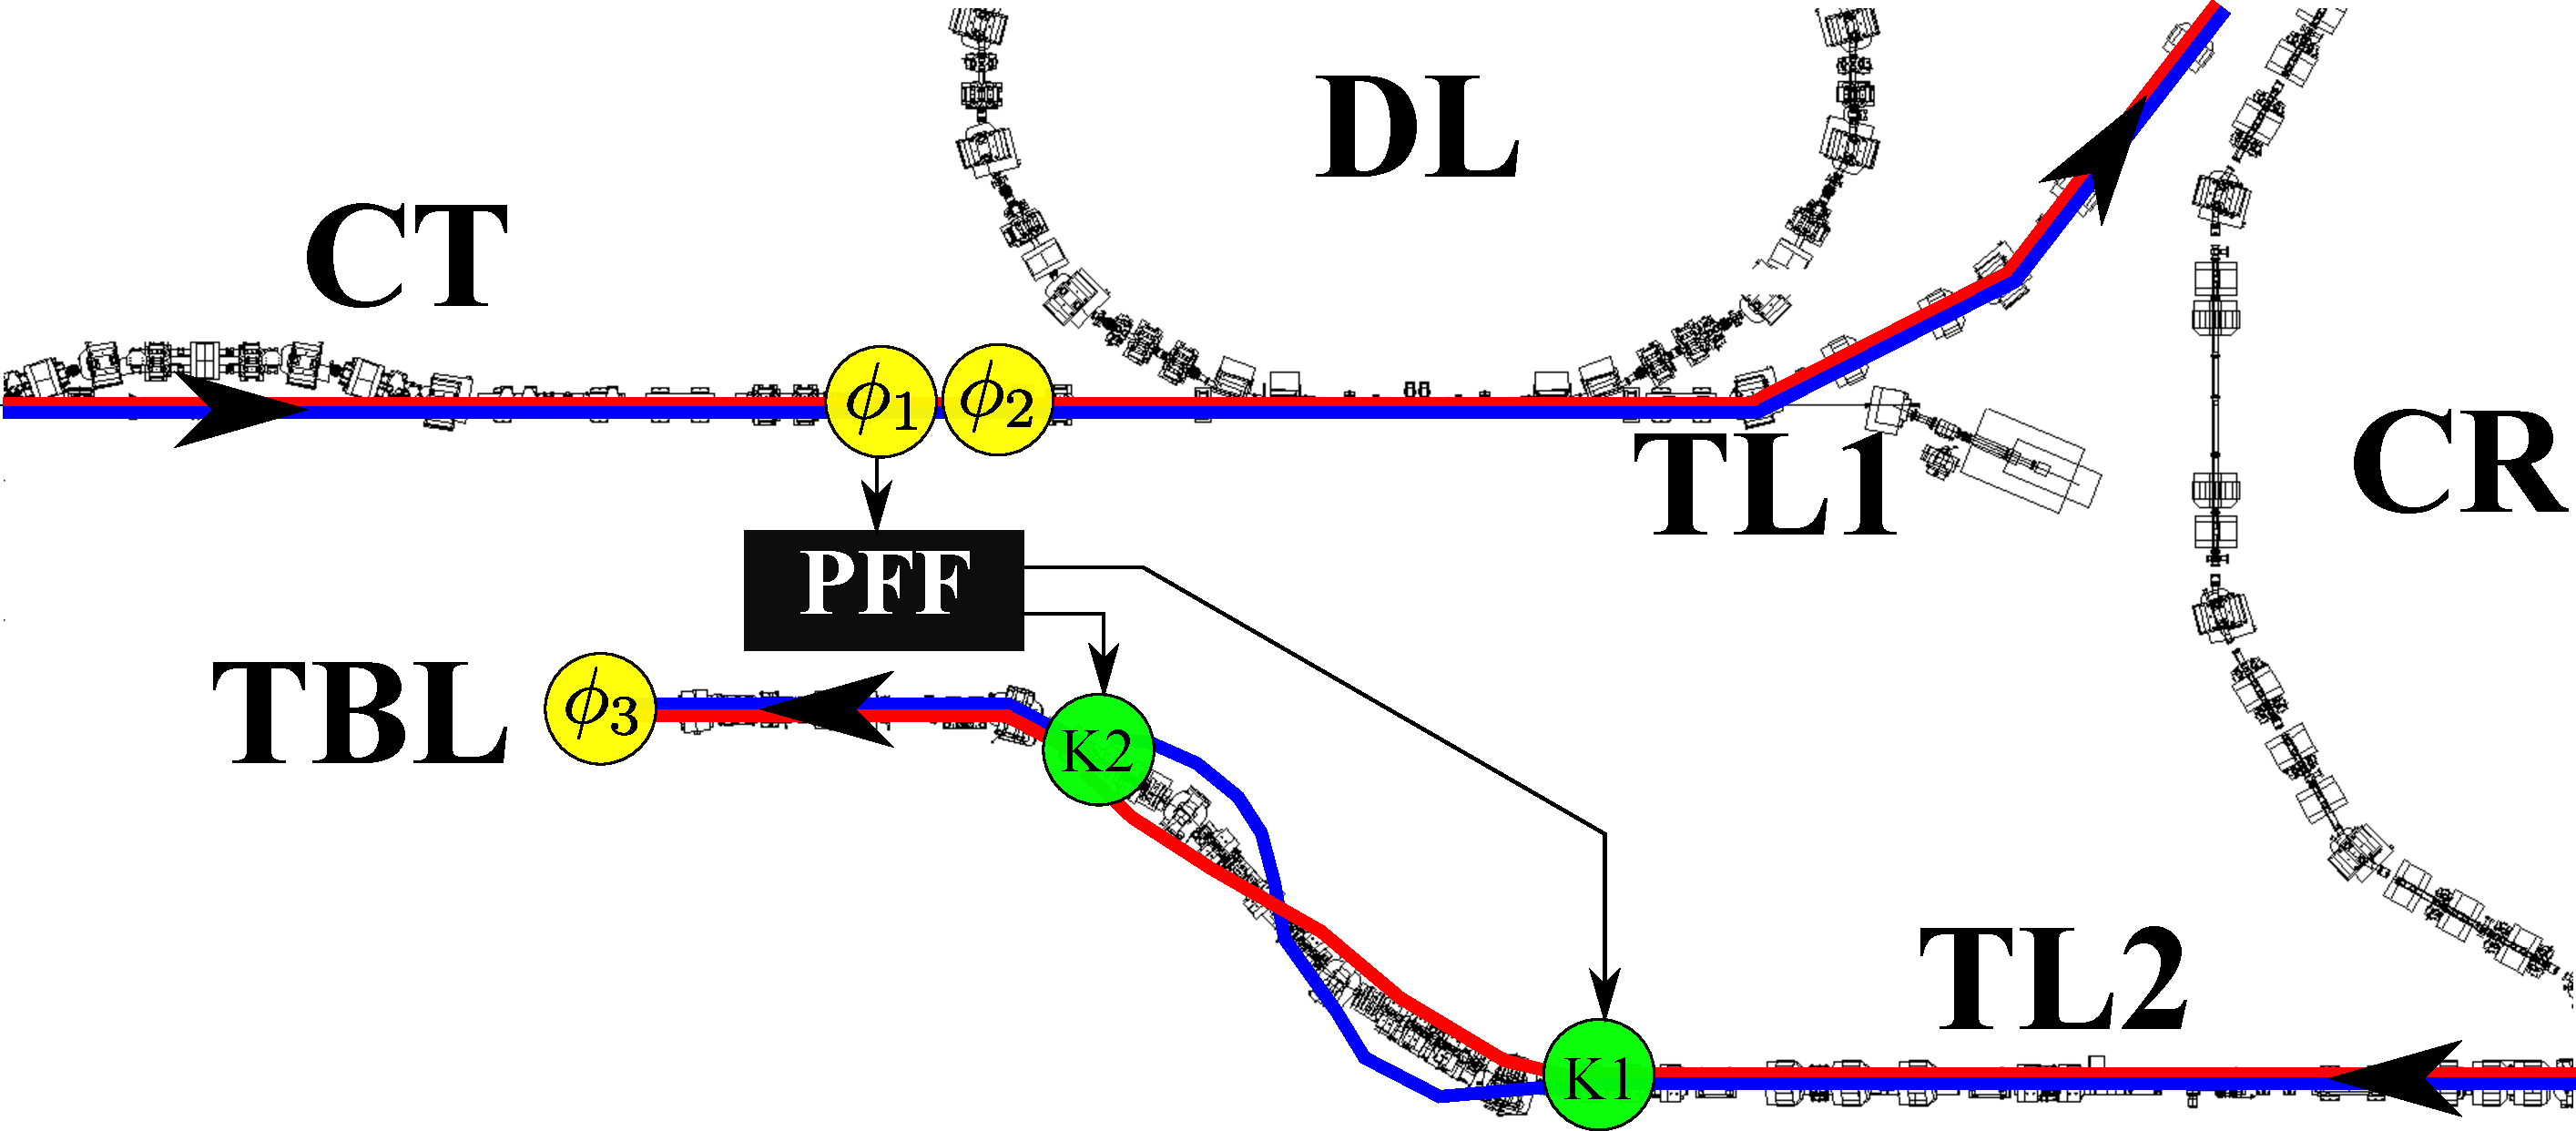
\includegraphics[width=\textwidth]{figs/ctfpffLayout}% Here is how to 
	%import EPS art
	\caption{\label{fig:pffLayout}Schematic of the PFF prototype at CTF3, 
	showing the approximate location of the phase monitors (\(\phi_1\) , 
	\(\phi_2\) and \(\phi_3\)) and
		the kickers (K1 and K2). The black box “PFF” represents the calculation 
		and output of the correction, including the phase monitor
		electronics, feedforward controller and kicker amplifiers. A bunch 
		arriving early at \(\phi_1\) is directed on to a longer path in the TL2 
		chicane
		using the kickers (blue trajectory), whereas a bunch arriving late will 
		be directed on to a shorter path (red trajectory). 
		\textcolor{red}{Maybe add upstream/downstream labels to phase monitors}}
\end{figure*}

A schematic of the PFF system is shown in Fig.~\ref{fig:pffLayout}. The system 
corrects the phase using two electromagnetic kickers installed 
before the first and last dipole in a four bend chicane (in the TL2 transfer 
line). The beam's path length 
through the chicane depends on the magnitude and polarity of the voltage 
applied to the kickers. The phase is measured using a monitor upstream of 
the chicane (in the CT beam line), and then corrected by setting the kicker 
voltage to deflect bunches arriving early at the phase monitor on to longer 
trajectories in the chicane, and bunches arriving late on to shorter 
trajectories. Downstream of the chicane, in the TBL line, another phase monitor 
is placed to measure the effects of the correction.

The beam time of flight between the upstream phase monitor and the first kicker 
in the chicane is 380~ns. By bypassing the combiner ring (CR) and TL1 transfer 
line, see Fig.~\ref{fig:pffLayout}, the total cable length required to 
transport signals between the monitor and kickers is shorter, approximately 
250~ns. The PFF correction in the chicane can therefore be applied to the same 
bunch initially measured at the phase monitor, providing the total system 
hardware latency is less than 130~ns. The system has a bandwidth of around 
30~MHz, able to remove phase variations along the 1.2~\(\mathrm{\mu s}\) CTF3 
beam 
pulse, as well as any offsets in the overall mean phase.


\subsection{\label{ss:hardware}Hardware}

The PFF system uses three phase monitors, two electromagnetic kickers, kicker 
amplifiers and a digitiser/feedforward controller.

The three phase monitors are designed and built by INFN Frascati, with the 
associated electronics built by CERN. The monitors are 12~GHz resonating 
cavities with a dipole and monopole mode present. The output from opposing 
vertical pairs of feedthroughs are summed in hybrids to create a position 
independent signal. This signal is split and mixed with a reference 12~GHz 
signal in eight separate mixers. The output from the eight mixers is combined, 
allowing a resolution of 0.126 degrees to be 
achieved whilst maintaining good linearity. This resolution is determined by 
comparing the measurements of the two monitors installed in the CT line.

The two electromagnetic kickers were also designed and built by INFN Frascati,  
and are based on the DAFNE design. A voltage of 1.26~kV applied to the 
downstream end of the kicker strips yields a horizontal deflection of 1~mrad 
for the 135~MeV CTF3 beam.

The kicker amplifiers have been designed and built by the John Adams 
Institue/Oxford University. For 
an input voltage of 2~V gives an output of up to 700~V. Response linear within 
3\% for input voltages up to \(1.2\)~V, then starts to saturate. Bandwidth 
47~MHz for small signal variations up to 20\% max output...

Finally, the Feedforward digitiser and controller (FONT5a board) was also 
designed and built by John Adams Institute/Oxford University. This takes the 
processed phase monitor signals then calculates and outputs the appropriate 
voltage with which to drive the amplifier. 9 ADCs, FPGA, 4 DACs... Digitises 
output from phase monitor electronics, calculates amplifier output based on set 
gain values, deals with correction timing...

The total latency of the phase monitor electronics, FONT5a board and amplifier 
is approximately 100~ns...

\subsection{\label{ss:optics}Chicane Optics}

The PFF system places additional constraints on the optics of the correction 
chicane, and also on the beam lines between the upstream phase monitor and the 
chicane. These constraints are needed to ensure a linear dependence of the 
phase on the kicker voltage, to ensure the PFF system does not degrade the beam 
orbit stability downstream of the chicane, and to ensure there is high 
correlation between the initial (uncorrected) upstream and downstream phase.

The correction range of the PFF system is defined by the kicker design, the 
maximum output voltage of the kicker amplifiers, and the optics transfer matrix 
coefficient \(R_{52}\) between the kickers in the chicane. The coefficient 
\(R_{52}\) describes the change in path length through the chicane per unit 
deflection at the first kicker. The optics at CTF3 have \(R_{52} = 0.74\)~m and 
at the maximum amplifier output 
of \(\pm700\)~V the kickers deflect the beam through 0.56~mrad. Together these 
define a correction range of approximately \(\pm400~\mathrm{\mu m}\), or 
\(\pm6\)~degrees, for the PFF 
prototype.

Fig. correction range...

\begin{figure}
	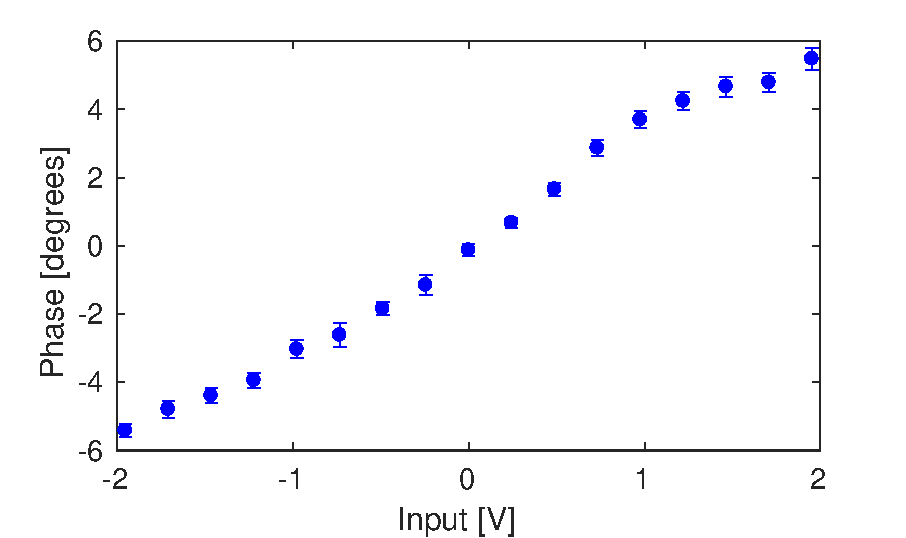
\includegraphics[width=0.5\textwidth]{figs/corrRange}
	\caption{\label{fig:corrRange}Correction range.}
\end{figure}

PFF system should not degrade transverse stability of beam after chicane. The 
purpose of the second kicker is to close the orbit bump created by the first 
kicker, so that the downstream beam orbit is independent of the kicker voltage. 
This can be achieved by requiring \(R_{11}=-1\) and \(R_{12}=0\) between the 
kickers...

\begin{figure}
	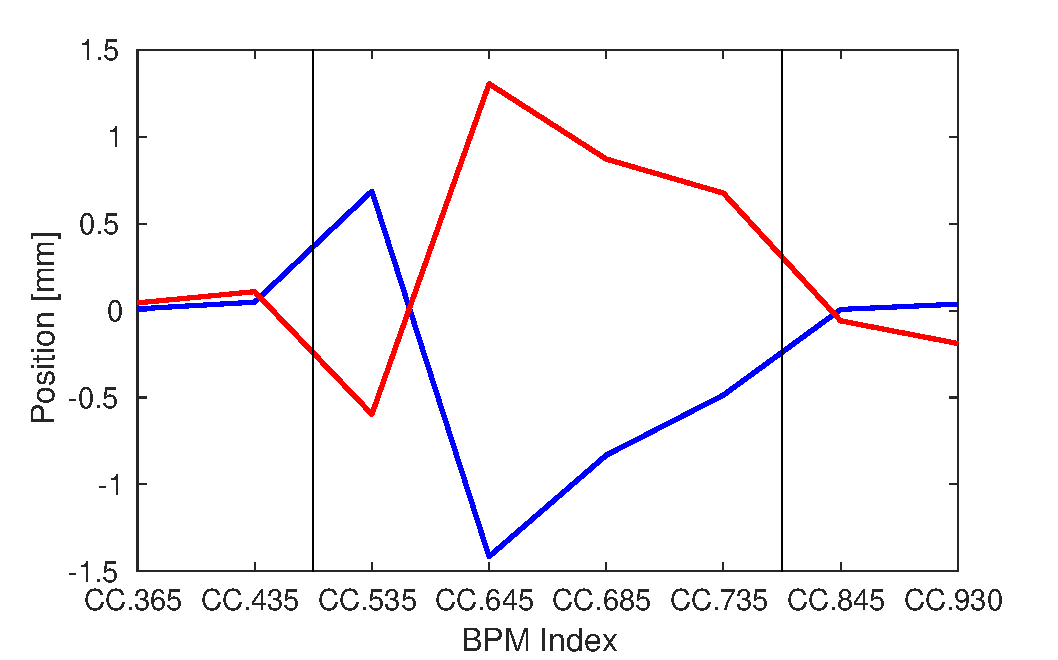
\includegraphics[width=0.5\textwidth]{figs/orbClos}
	\caption{\label{fig:orbClos}Orbit closure. \textcolor{red}{Maybe: Replace 
	lines with model 
	prediction, add lines to indicate kicker positions, remove -2 V 
	line}}
\end{figure}

All this must be achieved whilst keeping dispersion low, matching betas etc. 
within constraints of pre-existing buildings. Achieved R52 0.74m with max 
dispersion 1.16m...

\subsection{\label{ss:r56} Correlation}

The PFF system acts to subtract the measured upstream phase (\(\phi_u\)) from 
the initial downstream phase (\(\phi_d\)) with a gain factor (\(g\)):
%\begin{equation*}
\(\phi_{\mathrm{PFF}} = \phi_d - g\phi_u\)
%\end{equation*}
, where \(\phi_{\mathrm{PFF}}\) is the corrected downstream phase. The optimal 
system gain is given by:
\(g = \rho_{ud} \sigma_d/\sigma_u\)
, where \(\sigma_u\) and \(\sigma_d\) are the initial upstream and downstream 
phase jitter respectively, and \(\rho_{ud}\) is the correlation between the 
upstream and downstream phase. The theoretical limit on the corrected 
downstream phase jitter (\(\sigma_{\mathrm{PFF}}\)), with this gain is given by:
\(\sigma_{\mathrm{PFF}}=\sigma_d \sqrt{1-\rho_{ud}^2}\). 

One of the key challenges in operating the PFF prototype at CTF3 has been 
obtaining high correlation between the initial, uncorrected, upstream and 
downstream phase. A correlation of 97\% is required to reduce a typical initial 
phase jitter of \(0.8\)~degrees to the target of \(0.2\)~degrees. Early 
measurements showed only 40\% correlation.

The source of low correlation was discovered to be energy dependent phase 
jitter introduced between the upstream and downstream phase monitors. This is 
described via the optics transfer matrix coefficient \(R_{56}\):
\(\phi_d = \phi_u + R_{56}(\Delta p / p)\)
, where \(\Delta p / p\) is the relative beam energy offset.

Correlation vs. R56 equation?...

The PFF system requires \(R_{56}\) to be zero between the upstream and 
downstream phase monitors. All beam lines at CTF3 were nominally \(R_{56}=0\), 
but in the new PFF optics for the TL2 chicane a value of \(R_{56}=-0.18\)~m had 
to be tolerated, as it was not possible to meet all constraints for the line...

To compensate for the negative \(R_{56}\) in TL2, new sets of optics were 
created with positive \(R_{56}\) in TL1...

Figure R56...

\begin{figure}
	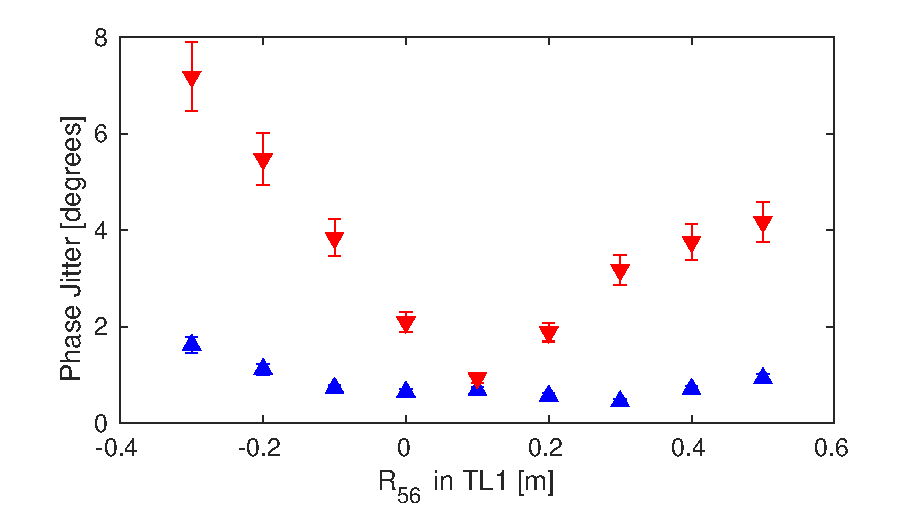
\includegraphics[width=0.5\textwidth]{figs/r56Scan}% Here is how to import 
	%EPS art
	\caption{\label{fig:r56Scan}R56 scan. \textcolor{red}{Maybe remove 
	upstream jitter.}}
\end{figure}


Higher order phase--energy dependencies and beam energy drifts at CTF3 
nevertheless mean it is difficult to maintain high correlation between the 
upstream and downstream phase on long timescales...

\section{\label{s:results}Results}

\subsection{\label{ss:gScan}Gain Scan}

With the optimal gain the PFF correction acts to remove all correlation between 
the upstream and downstream phase, reducing the downstream phase jitter. If the 
gain is too small some residual correlation will remain, and if it is too large 
the correlation will flip sign. 

The optimal system gain can be derived empirically by observing the dependence 
of the downstream phase on the upstream phase with the correction on, as seen 
in Fig.~\ref{fig:gScan}.

\begin{figure}
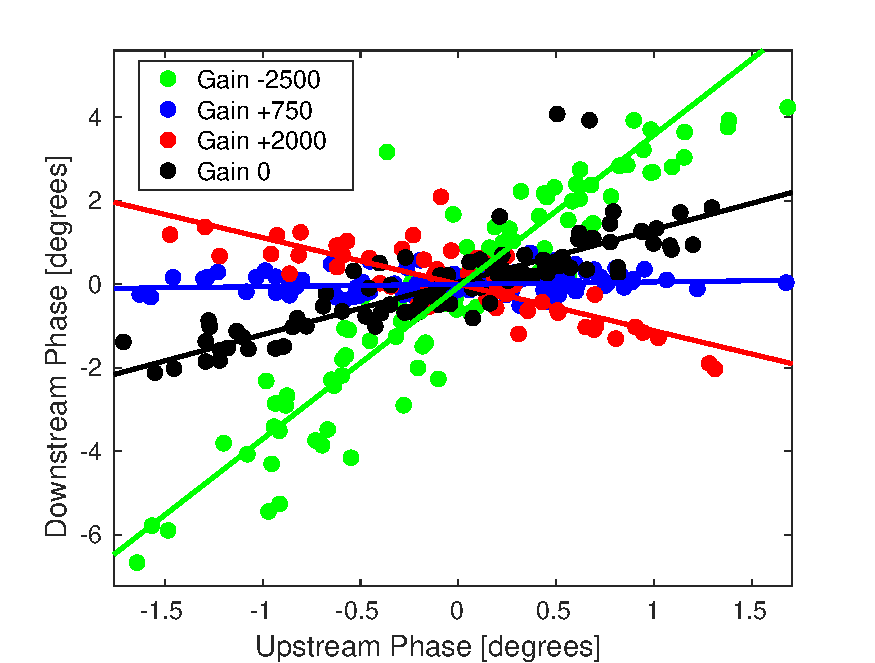
\includegraphics[width=0.5\textwidth]{figs/gScan}% Here is how to import EPS art
\caption{\label{fig:gScan}Gain scan. \textcolor{red}{Look for better data. 
And/or convert to real gain from FONT gain.}}
\end{figure}


\subsection{\label{ss:meanJit}Pulse-to-pulse Jitter}

The mean phase is defined as: mean phase across xxx~ns portion of pulse, for 
each pulse.

Fig.~\ref{fig:meanJit} shows a ten minute dataset (xxx pulses), in which an 
initial mean phase jitter of 0.92~degrees is reduced to 0.20~degrees by the PFF 
correction. The system is operated in interleaved mode, with the correction 
applied to alternating pulses, so that a measurement of the initial and 
corrected downstream phase jitter can be performed at the same time.

All correlation between the upstream and downstream jitter is removed, from 
96\% to 0\%. 

Across 20 minutes, 0.30 degrees phase jitter has been achieved.

Best result:
\(0.92\pm0.04^\circ\) to \(0.20\pm0.01^\circ\)  across 10 minutes,
Correlation \(96\pm2\%\) to \(0\pm7\%\),
Theoretical limit: \(0.26\pm0.06^\circ\),
NB: upstream PFF off is \(0.76\pm0.03^\circ\), but \(0.68\pm0.03^\circ\) for 
PFF on.


\begin{figure}
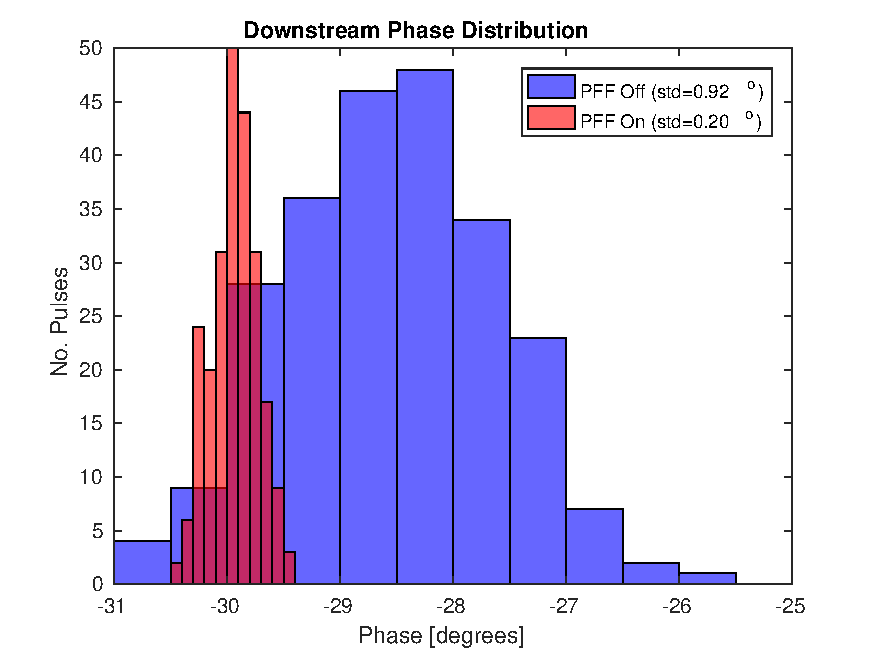
\includegraphics[width=0.5\textwidth]{figs/BestFF_meanJit}% Here is how to import EPS art
\caption{\label{fig:meanJit}Best mean phase jitter. 0.92 degrees to 0.20 
degrees.}
\end{figure}


\subsection{\label{ss:shape}Intra-Pulse Phase Variations}

High bandwidth correction - not only correcting the mean but also variations 
along the pulse...

OLD VALUES: (Peak-to-peak variation of 5.76 degrees in initial phase reduced to 
0.65 degrees in corrected phase -- OR -- standard deviation of phases reduced 
from 1.68 to 0.26 degrees...). Current figure is worse.

Histogram: improvement in flatness.

\begin{figure}
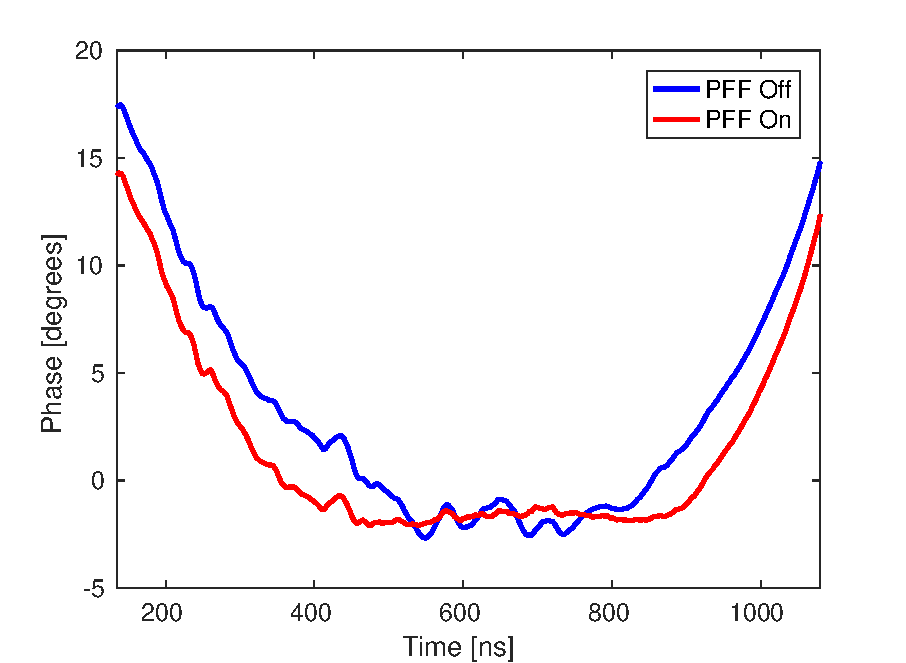
\includegraphics[width=0.5\textwidth]{figs/BestFF_shape}% Here is how to import EPS art
\caption{\label{fig:shape}Correction of pulse shape - look for better data.}
\end{figure}

\subsection{\label{ss:pbpJit}Point-by-point Jitter}

\textcolor{red}{I think this can probably be removed. Not sure it adds any 
information beyond mean jitter and correction of shape. Would remove this 
section, replace plot with histogram of improvement in shape.}

\begin{figure}
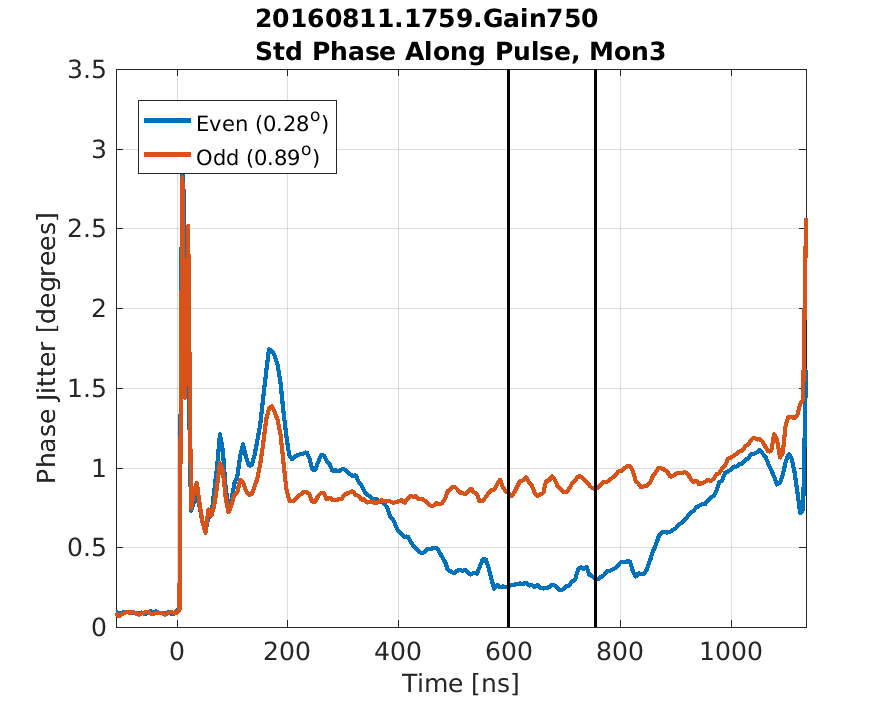
\includegraphics[width=0.5\textwidth]{figs/BestFF_pbp}% Here is how to import EPS art
\caption{\label{fig:BestFF_pbp}Point-by-point jitter.}
\end{figure}


Point-by-point jitter of x~degrees achieved across a x~ns portion of the pulse, agrees with simulated value...

Limited by variations in phase propagation along the pulse (energy differences etc.), plus resolution slightly worse for point by point than for mean.



\section{\label{s:conc}Conclusions}

CLIC requires a PFF system to reduce the drive beam phase jitter by an order of 
magnitude, from 2.0~degrees to 0.2~degrees. A prototype of the system has been 
in operation at the CLIC test facility CTF3.

The prototype has demonstrated \(0.20\pm0.01^\circ\) pulse-to-pulse 
phase jitter on a time scale of ten minutes. 

Intra-pulse phase variations are also greatly reduced by the PFF system...

Drifts, in particular in beam energy, degrade the correlation between the 
upstream and downstream phase and prevent this level of stability from being 
demonstrated on longer time scales at CTF3. A key consideration for any future 
system should be to design beam lines and optics with zero phase-energy 
dependence, including non-linear dependencies, to solve this issue.

Try to apply to XFELs/something else.

\bibliography{apssamp}% Produces the bibliography via BibTeX.

\end{document}
